\documentclass[aspectratio=169]{beamer}
\def\ntitle {Geometric Mechanics on Diffeomorphisms\\[0.1cm] {\small A view into conservation arising from Geometry}} % Title of the Document
\def\shorttitle {GeomMechDiff} % Short title for bottom of slides
\def\nauthor {James Arthur} % Author of slides
\def\nposition {MSc Mathematical Modelling and Scientific Computing} % Position in dept.
\def\nname {Dissertation Viva 2023} % name of where you are presenting
\def\ndate {September 2023} % Date

\usepackage{ox_temp}
\usepackage{beamer_preamble}


\usepackage{biblatex}
\addbibresource{refs.bib}


\AtBeginSection[]
{
    \begin{frame}
        \frametitle{Table of Contents}
        \tableofcontents[currentsection]
    \end{frame}
}

\usepackage{epigraph}
\renewcommand{\epigraphflush}{center}

%% Content of slides %%

\begin{document}
    \begin{frame}[plain]
        \titlepage
    \end{frame}
    %

    \frame{
    \frametitle{Aims of this thesis}
      We aim to study an area of mathematics that lies behind Numerical Analysis for structure preserving numerical methods. In this presentation we will look at three things,
      \begin{itemize}
        \item Motivation via a structure preserving numerical method,
        \item Main results, such as Euler-Poincar\'e reduction, Lie-Poisson reduction and Noether Theorems.
        \item Some problems faced, and further work.
      \end{itemize}
    }

    \frame{
    \frametitle{Motivation}
    \framesubtitle{Numerical Results}
    \begin{figure}
      \vspace{10pt}
      \centering
      \begin{minipage}{.5\textwidth}
        \centering
        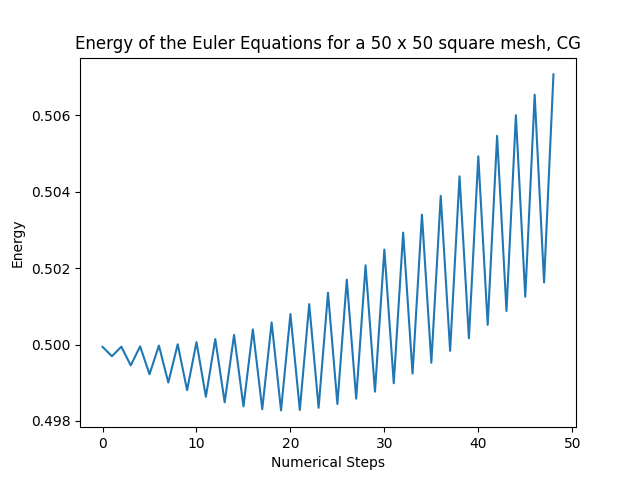
\includegraphics[width=.9\linewidth]{./img/energy.png}
        \label{fig:test1}
      \end{minipage}%
      \begin{minipage}{.5\textwidth}
        \centering
        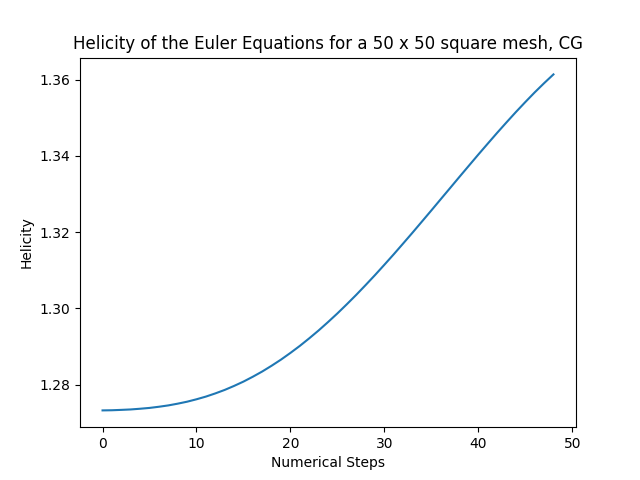
\includegraphics[width=.9\linewidth]{./img/helicity.png}
        \label{fig:test2}
      \end{minipage}
      \caption{Conservation Quantities of the Euler Equations}
    \end{figure}
    }

    \frame{
    \frametitle{Motivation}
    \framesubtitle{Error}
      A lot of the error above comes from spatial error as we use a midpoint scheme in the temporal steps, which is symplectic. Hence we need to discretise the spatial steps symplectically.
    }

    \frame{
    \frametitle{Motivation}
    \framesubtitle{Poisson Bracket Schemes}
      Any Hamiltonian system can be written as,
      $$ \di F t = \{F,\, H\}. $$
      The Lie-Poisson (or Poisson) bracket holds a lot of conservation properties, hence if we can discretise this such that $\{\cdot ,\, \cdot\}_D$ still has these properties then we have a symplectic spatial discretisation.
    }

    \frame{
    \frametitle{Motivation}
      My thesis aims to answer the questions,\vspace{20pt}
      \begin{center}
        \textit{What are these properties? How can we characterise these types of brackets and how does this all apply to fluid dynamics? Can we generalise this theory?}
      \end{center}
    }

    \frame{
    \frametitle{Main Results}
    \framesubtitle{Classical Mechanics}

    \begin{figure}[!ht]
    \centering
    \vspace{40pt}
    \rotatebox[origin=c]{270}{
    \resizebox{0.35\textwidth}{!}{\input{./img/legendre.pdf_tex}}
    }
    \label{fig:diffeos}
    \end{figure}
    }

    \frame{
    \frametitle{Main Results}
    \framesubtitle{Lagrangian Mechanics}
    \vspace{20pt}
    \begin{nthm}[Euler-Lagrange Theorem~\cite{imas}]
      Let $G$ be a Fr\'echet Group and $ L : TG \to \R $ be a Lagrangian. Then the following are equivalent,
      \begin{itemize}
        \item Hamiltons Principle with endpoint conditions, $\d {\vec q}(t_1) = \d {\vec q}(t_2) = 0$,
        $$ \d \int_{t_1}^{t_2} L({\vec q},\, \dot {\vec q}) \, \dd t = 0 $$
        \item The Euler-Lagrange equations,
        $$ \dit \pd L {\vec {\dot q}} - \pd L {\vec q} $$
      \end{itemize}
    \end{nthm}

    }

    \frame{
    \frametitle{Main Results}
    \framesubtitle{Reduced Mechanics}

    When we consider a symmetry we can reduce the Lagrangian by a copy of $G$. This is called the `reduced' Lagrangian.
    $$ \ell : (TG / G) \to \R. $$
    We note $(TG / G) \cong \frg$.
    }

    \frame{
    \frametitle{Main Results}
    \framesubtitle{Basic Euler-Poincar\'e}
    \vspace{20pt}
    \begin{nthm}[Basic Euler-Poincar\'e Theorem  ~\cite{holm}]
      Let $G$ be a Fr\'echet Group and $ \ell : \frg \to \R $ be a Lagrangian. Then the following are equivalent,
      \begin{itemize}
        \item Hamiltons Principle and the reduced action principle with endpoint conditions, $\d {\vec q}(t_1) = \d {\vec q}(t_2) = 0$.
        \item The Euler-Lagrange Equations.
        \item The Basic Euler-Poincare equations where, $\d \vec u = \dot {\vec u} + [\vec w,\, \vec u]$,
        $$ \pd{}{t} \fd \ell {\xi} + \ad^*_\xi \fd \ell {\xi} = 0. $$
      \end{itemize}
    \end{nthm}
    }

    \frame{
    \frametitle{Main Results}
    \framesubtitle{Advected Euler-Poincar\'e}
    \vspace{20pt}
    \begin{nthm}[Advected Euler-Poincar\'e Theorem ~\cite{holm}]
      Let $G$ be a Fr\'echet Group, $ \ell : \frg \rtimes V^* \to \R $ be a Lagrangian and $a \in V^*$ be an advected parameter living in the dual of a representation space, $V^*$. Then the following are equivalent,
      \begin{itemize}
        \item Hamiltons Principle and the reduced action principle with endpoint conditions, $\d {\vec q}(t_1) = \d {\vec q}(t_2) = 0$.
        \item The Euler-Lagrange Equations for $L_{a_0}$.
        \item The Advected Euler-Poincare equations where, $\d \vec u = \dot {\vec u} + [\vec w,\, \vec u]$,
        $$ \pd{}{t} \fd \ell {\xi} + \ad^*_\xi \fd \ell {\xi} = \fd \ell a \diamond a \qquad \left( \pd{}{t} + \mathcal{L}_\xi \right)a = 0. $$
      \end{itemize}
    \end{nthm}
    }

    \frame{
    \frametitle{Main Results}

    If we let the Lagrangian be,
    $$ L = \int_M |\dot \eta|^2\mu. $$
    Then reduction under relabelling symmetry produces,
    $$ \ell = \int_M |\vec u|^2 \mu, $$
    where $\vec u = \dot \eta \eta^{-1}$.
    }

    \frame{
    \frametitle{Main Results}
    \framesubtitle{Conservation}
    Then the basic Euler-Poincar\'e equations produce the Euler's Equations for ideal fluid flow. We can now try and find conserved quantities for these equations.
    }

    \frame{
    \frametitle{Main Results}
    \framesubtitle{Noether Theorem}
    \begin{align*}
      0 &= \int_{t_1}^{t_2} \int_M \ip{\fd \ell {\vec u}}{\pd \nu t} - \ip{\ad^*_{\vec u} \fd \ell {\vec u}}{\nu} + \ip{a \diamond \fd \ell a}{\nu} \dd t \\
      &= \int_{t_1}^{t_2} \int_M \ip{-\pd{}{t}\fd \ell {\vec u} - \ad^*_{\vec u} \fd \ell {\vec u} + a \diamond \fd \ell a}{\nu} \dd t + \int_M\left. \ip{\fd \ell {\vec u}}{\nu}\right|_{t_1}^{t_2} \mu \\
      &= \int_M \left.\ip{\fd \ell {\vec u}}{\nu}\right|_{t_1}^{t_2} \mu.
    \end{align*}

    }

    \frame{
    \frametitle{Main Results}
    \framesubtitle{Noether Theorem}
    \begin{nthm}[Noether Theorem]
      Let $G$ be a Fr\'echet Group and $\ell : \frg \rtimes V^* \to \R$ be a reduced advected lagrangian. Then the following is conserved,
      $$ \dit \int_M \ip{\fd \ell {\vec u}}{\nu}\mu = 0.$$

    \end{nthm}

    }

    \frame{
    \frametitle{Problems Faced}
    \framesubtitle{A lot of low hanging fruit no longer exists}
    This area is based on Differential Geometry, an area famed for being hard to learn and even harder to add new contributions to. Most of Geometric Mechanics is already studied in papers of 50 pages in length, mostly regurgitating the same material. This makes it very hard to make new contributions. Theoretically there is little to do, so most of the contributions are in our examples, by clearly laying them out in terms not done before.
    }

    \frame{
    \frametitle{Problems Faced}
    \framesubtitle{A high barrier to entry}
    In order to study and produce new research in this area you first need to understand the preceding work. This area has been developed over several years and with me and my supervisor green to continua reduction over manifolds we have had to learn from papers and build up the theory from scratch.
    }

    \frame{
    \frametitle{Problems Faced}
    \framesubtitle{No set endpoint}
    We never set an endpoint or a goal. The goal was to investigate this mathematics and hope we find something interesting along the way. This may make the dissertation look scattered as I did a wide variety of things as I tried to tie together all my skills from MMSC.
    }

    \frame{
    \frametitle{Further Work}
    \framesubtitle{Poisson Bracket Schemes}
    \vspace{20pt}
    We can apply this theory to more than ideal fluids. Consider the shallow water equations, then the Arnold Bracket is~\cite{salmonps},
    $$ \{F, G\} = \int_M \left( \fd {(F,\, G)} {(u,\, v)} - \fd F {\vec u} \cdot \nab \fd G h + \fd G {\vec u} \cdot \nab \fd F h  \right) \dd x. $$
    In 1D we can discretise,
    \begin{align*}
      \{f, g\}_D = \sum_i \frac{1}{2\D} & \frac{v_{i+1} - v_{i-1}}{h_i} \fd {(f,\, g)} {(u_i,\, v_i)} - \fd f {u_i} \left( \fd g {h_{i+1}} - \fd g {h_{i-1}} \right)\\
      &+ \fd g {u_i} \left( \fd f {h_{i+1}} - \fd f {h_{i-1}} \right).
    \end{align*}
    }

    \frame{
    \frametitle{Further Work}
    \framesubtitle{More Generally...}
    In the wider picture we can dive more deeply into the Symplectic property of this area. We can study symplectic and multisymplectic reduction that leads to a theory of waves. Further we can study how these waves interact with rigid bodies and then we arrive in the area of my PhD.

    }

    \begin{frame}[plain,allowframebreaks]\vspace{10pt}
    \frametitle{References}
    \printbibliography
    \end{frame}

    \begin{frame}\vspace{30pt}
      \begin{center}
        {\huge Fin}\\\vspace{20pt}
        {\huge Questions?}
      \end{center}
    \end{frame}

\end{document}